% Evidence fragment: include in the orbital chapter. Retained booktabs,
% tabularx/Y, graphicx, hyperref and xurl suffice; no new packages.
\subsection{R2 physical-position results and separate confirmation}
\label{sec:orbit-validation}

The R2 models stay below the adopted \textbf{10 m three-dimensional
reference-discrepancy budget at every tested sample through 24 hours} for all
four targets, on both the January benchmark and the separate February
confirmation date. This statement concerns sampled positions of these seeds;
it is not a universal or continuous-time orbit guarantee.
The January window was previously inspected during R1 development and is
explicitly a \textbf{reused benchmark}. The February selection procedure was
frozen before its future errors were evaluated; no model was retuned afterward.

The forecast quantity is
\[
 e_i=\|\widehat{\boldsymbol r}(t_i)-\boldsymbol r_{\rm reference}(t_i)\|_2,
 \qquad t_i>t_0.
\]
The January origin is 2 January 2025 00:00 GPST,
$t_0=1419811200$; February uses 2 February 2025 00:00 GPST,
$t_0=1422489600$. All cutoff and earlier target rows are excluded from the
forecast curves. R2 selects among 1-, 3- and 7-day training windows using an
internal validation day entirely before the forecast origin. The selected
January windows are 3/3/3/1 days for G05/C03/C06/Chandra; the unchanged rule
selects 1/7/3/3 days for February. External EGM96 gravity and planetary forcing
are distinct from future target observations.

\begin{table}[htbp]
\centering\small
\caption{Maximum discrepancy over all first-day samples (metres). Each R2
column has 288 samples per target through 24 h; Chandra's final sample is
approximately 51.185 s before the exact endpoint.}
\label{tab:orbit-first-day-comparison}
\begin{tabular*}{\linewidth}{@{\extracolsep{\fill}}lrrr@{}}
\toprule
Target & R1 January & R2 January & R2 February\\
\midrule
G05 / MEO & 285.330 & 1.057 & 3.072\\
C03 / GEO & 20.600 & 5.304 & 4.654\\
C06 / IGSO & 44.684 & 1.172 & 2.108\\
Chandra / HEO & 76.506 & 8.093 & 0.290\\
\bottomrule
\end{tabular*}
\end{table}

\begin{table}[htbp]
\centering\small
\caption{R2 January discrepancy in metres at the nearest actual sample to each
requested horizon. Individual samples are not worst-case interval errors.}
\label{tab:orbit-horizon-samples}
\begin{tabular*}{\linewidth}{@{\extracolsep{\fill}}lrrrrrr@{}}
\toprule
Target & 15 min & 1 h & 6 h & 24 h & 72 h & 7 d\\
\midrule
G05 / MEO & 0.474 & 0.655 & 0.272 & 0.713 & 2.228 & 12.531\\
C03 / GEO & 1.368 & 1.702 & 4.350 & 4.172 & 17.939 & 73.481\\
C06 / IGSO & 0.547 & 0.609 & 0.615 & 1.172 & 2.335 & 2.360\\
Chandra / HEO & 0.003 & 0.008 & 0.074 & 2.052 & 28.338 & 3680.247\\
\bottomrule
\end{tabular*}
\end{table}

\textbf{Time grid.} GNSS is on the exact requested GPST grid. Chandra is supplied
on a 300 s TDB grid, converted using the periodic TDB--TT correction and
$\mathrm{GPST}=\mathrm{TT}-51.184\,\mathrm{s}$. The nearest 15 min sample is
848.816057 s after the January origin and 848.815204 s after the February
origin. The final samples are respectively 604748.815856 s and
604748.815036 s. Exact offsets remain in the CSV/JSON, including all six
requested horizons for both dates.

\begin{table}[htbp]
\centering\small
\caption{R2 whole-window statistics (metres). January has 2,016 samples per
target. February has 2,016 each except C03, which has 1,441 and a 48 h gap.}
\label{tab:orbit-period-errors}
\begin{tabular*}{\linewidth}{@{\extracolsep{\fill}}lrrrr@{}}
\toprule
Target & Jan. RMS & Jan. maximum & Feb. RMS & Feb. maximum\\
\midrule
G05 / MEO & 5.294 & 12.998 & 33.113 & 71.800\\
C03 / GEO & 37.434 & 78.717 & 39382.862 & 100604.174\\
C06 / IGSO & 2.943 & 8.084 & 3.494 & 7.629\\
Chandra / HEO & 5412.235 & 25635.951 & 2055.685 & 5663.182\\
\bottomrule
\end{tabular*}
\end{table}

The seven-day 10 m budget is \textbf{not met for all targets}. C06 stays
below it at every seven-day sample on both dates; G05 exceeds it later on both
dates. C03 and Chandra have additional reference qualifications below.
The original R1 seven-day maxima were 7402.960/532.582/1237.242/19399.307 m
in the same object order. The R2 first-day improvement must not be extended
into a claim that every seven-day maximum improved or passed.
RMS and percentiles describe correlated samples, not independent-sample
confidence intervals. Reports additionally retain interval RMS/maxima and
sample percentiles.

\subsection{Sampled thresholds and incomplete reference coverage}
\label{sec:orbit-thresholds}
\begin{table}[htbp]
\centering\small
\caption{Preceding sample and first sampled exceedance, in hours after the
origin, rounded to 0.001 h. These pairs are not certified continuous crossing
brackets. ``None'' means no exceedance at the available samples.}
\label{tab:orbit-first-exceedance}
\begin{tabularx}{\linewidth}{@{}llYYY@{}}
\toprule
Date & Target & 10 m & 100 m & 1 km\\
\midrule
January & G05 / MEO & $(145.083,145.167]$ & None at samples & None at samples\\
January & C03 / GEO & $(29.000,29.083]$ & None at samples & None at samples\\
January & C06 / IGSO & None at samples & None at samples & None at samples\\
January & Chandra / HEO & $(50.402,50.486]$ & $(82.569,82.652]$ & $(83.986,84.069]$\\
February & G05 / MEO & $(50.833,50.917]$ & None at samples & None at samples\\
February & C03 / GEO & $(72.000,120.000]$ & $(72.000,120.000]$ & $(72.000,120.000]$\\
February & C06 / IGSO & None at samples & None at samples & None at samples\\
February & Chandra / HEO & $(83.986,84.069]$ & $(83.986,84.069]$ & $(83.986,84.069]$\\
\bottomrule
\end{tabularx}
\end{table}

For 10 km, January Chandra first exceeds the level at 302648.815956 s,
following the sample at 302348.815956 s; all January GNSS targets remain below
10 km at their samples. February C03 first exceeds 10 km at the first sample
after its gap, 432000 s; the previous sample is at 259200 s. Other February
targets remain below 10 km at the sampled times.

\textbf{C03 February coverage.} GFZ contains no C03 records on February 5 and
6. Adjacent daily endpoints leave a 48-hour reference gap and 575 missing
five-minute samples. Wuhan also lacks C03 on February 6 and cannot certify the
missing interval. GFZ remains the predeclared primary source. The first
post-gap discrepancy is 29256.547 m and the later maximum is 100604.174 m;
these observed exceedances are retained. Full-window coverage is
\textbf{indeterminate}, and no continuous tolerance passage through the gap is
inferred. No maneuver or other cause is assigned from missing records alone.
The figures leave the missing interval blank.

\subsection{Numerical error and reference discontinuities}
\label{sec:orbit-error-separation}
\begin{table}[htbp]
\centering\small
\caption{Separate numerical and frame comparisons, in metres. January's
independent physical audit uses 11 times across the past/future domain;
February compares nine future checkpoints with adaptive DOP853. The frame
column is the larger of the two complete sampled frame-approximation maxima.}
\label{tab:orbit-error-components}
\begin{tabular*}{\linewidth}{@{\extracolsep{\fill}}lrrr@{}}
\toprule
Target & Jan. RK4/DOP853 & Feb. RK4/DOP853 & Frame approximation\\
\midrule
G05 / MEO & 0.031716 & 0.026461 & 0.002007\\
C03 / GEO & 0.001232 & 0.001023 & 0.003260\\
C06 / IGSO & 0.001252 & 0.001026 & 0.003169\\
Chandra / HEO & 0.036582 & 0.147044 & 0.009135\\
\bottomrule
\end{tabular*}
\end{table}

Native RK4 uses 30 s for GNSS and 7.5 s for Chandra. Same-seed integration
agreement tests arithmetic, not orbit truth. The January forecast report's
own DOP853 check covers only its first sample; the wider January evidence above
comes from the separate, target-independent physical audit. Native CPU/CUDA
checks and exact word/packing checks remain separate evidence.
The frame test compares the embedded daily-EOP/Chebyshev frame with direct SOFA
IAU 2006/2000A evaluation of the same published prediction. It excludes actual
future EOP error, station uncertainty and a complete relativistic ICRF/GCRS
coordinate error budget; it is not subtracted as an independent scalar variance.

\begingroup\clubpenalty=10000
\textbf{Chandra source discontinuities.} The January error rises from
123.204 m to 23839.033 m between two five-minute samples. A separate one-second
Horizons query shows that at January 5 TDB 12:01:09--12:01:10 the source
position displacement differs from the integral of its own reported velocity
by \textbf{24317.077 m}; outside the neighboring jump intervals the same local
check is at most 0.0654 m. Native RK4 agrees with independently tightened
DOP853 to about 1.5 mm at the two forecast endpoints surrounding that jump.
The source header identifies CFA's merged trajectory, but no local join or
maneuver cause. The large discontinuity therefore cannot be attributed solely
to smooth force error or native integration.
\par\endgroup

The February reference has a corresponding kinematic discontinuity at
February 5 TDB 12:01:09--12:01:10: \textbf{2487.123 m} displacement-minus-velocity
integral mismatch, versus at most $2.26\,\mu\mathrm{m}$ away from its neighboring
intervals. The forecast's next five-minute error rises from 1.053 m to
2492.098 m. These diagnostics use only the source's positions and velocities;
no model is fitted to them. \textbf{All original discrepancy samples and
whole-window maxima are retained.} The cause of the provider discontinuities
is not established, and no corrected ``true orbit'' accuracy is invented.
Original queries, hashes and calculations are in
\path{source/orbit_data/diagnostics/}.

\textbf{Reference uncertainty.} January GFZ/Wuhan comparisons give 3D RMS
0.0263 m for G05, 2.074 m for C03 and 0.1692 m for C06; C03's maximum provider
disagreement is 3.575 m. These are product differences, not certified absolute
bounds. Providers share some underlying observations. Chandra supplies no
state covariance or absolute position guarantee. A millimetre or sub-metre
match to a selected reference is therefore not a matching physical-accuracy
claim.

\subsection{Chronology, source conventions and reproducible evidence}
\label{sec:orbit-provenance}
The R2 physical model uses the documented degree/order-12 EGM96 field,
cutoff-available daily Earth orientation, and external Sun/Moon forcing.
EGM96's original mu, reference radius, tide-free convention and fully normalized
coefficients are preserved with explicit conversion in
\path{source/orbit_data/gravity_reference/}. The format's normalization default
is documented by ICGEM:
\url{https://icgem.gfz.de/docs/ICGEM-Format-2023.pdf}.

The EOP sources were published before their cutoffs: IERS Bulletin A of
26 December 2024 and 30 January 2025, respectively:
\url{https://datacenter.iers.org/data/6/bulletina-xxxvii-052.txt} and
\url{https://datacenter.iers.org/data/6/bulletina-xxxviii-005.txt}.
Both permit public release and unlimited distribution.
The February GFZ reference changes from IGS20 to IGb20. IGSMAIL-8543, published
9 December 2024, specifies zero datum transformation parameters because origin,
scale and orientation remain aligned; individual reference-station coordinates
are updated. Preserve each source label and apply no fitted alignment:
\url{https://lists.igs.org/pipermail/igsmail/2024/008539.html}.

Precise target products were retrieved retrospectively; their earlier estimates
can incorporate later observations within provider processing. Neither date
proves that identical seeds were available live in 2025. January is a reused
comparison, while February applies the already-frozen selection rule to a
separate date. The confirmation freeze manifest binds the rule and model-file
hashes. Raw source acquisition and coverage inspection preceded any February
prediction-error evaluation. No later error was used to refit a seed.

\begin{itemize}
\item \textbf{GFZ and IGS.} Retain GFZ/IGS provider and network attribution.
The cited GFZ product-series DOI is
\url{https://doi.org/10.5880/GFZ.1.1.2016.003}; its DataCite record declares
\textbf{CC BY-NC 4.0}. The DOI names an ultra-rapid series whereas these GBM
files are rapid products without a separate per-file grant. The fixture bundle
conservatively retains that noncommercial qualification and is not claimed as
unrestricted commercial data. IGS terms:
\url{https://www.igs.org/wp-content/uploads/2020/09/IGS-Data-and-Product-Disclaimer-and-Terms-of-Use-200805.pdf}.
\item \begin{minipage}[t]{\linewidth}\textbf{CODE and Wuhan.} CODE's reference
\url{https://doi.org/10.48350/197028} lists open access/BORIS terms, not a blanket
MIT grant. Wuhan final products retain provider/IGS attribution. Original
archive URLs and per-file hashes remain in the source manifests.\end{minipage}
\item \textbf{NASA/JPL and CFA.} Acknowledge Giorgini and the JPL Solar System
Dynamics Group, NASA/JPL Horizons, and CFA for Chandra:
\url{https://ssd.jpl.nasa.gov/horizons/}.
Retrieval date is 15 September 2026. Geometric ICRF/TDB settings and original
responses are retained. Sun/Moon Horizons responses identify DE441; the
construction oracle is DE440s, a distinct planetary ephemeris version.
\end{itemize}

\textbf{Authoritative reports.} Use
\path{results/orbit_accuracy_r2_cpu_verified/accuracy_summary.json}, its CUDA
counterpart, and
\path{results/orbit_accuracy_confirmation_cpu_verified/accuracy_summary.json}.
R1 evidence remains in \path{results/orbit_accuracy_cpu_final/} for comparison.
The pre-fix failed trial and superseded intermediate models are not final
accuracy evidence. CSVs retain every measured error, exact horizon offset,
source and frame. Each report distinguishes \path{model_file_sha256} from
\path{physical_model_sha256}=\path{orbit_seed.digest(model)}; legacy
\path{model_sha256} is explicitly the file-hash alias. Accuracy displayed for a
custom packed seed applies only when the physical-model digest matches.
Reference fixtures, publications and the DE440s construction binary are
separate from the complete replay seed byte count.

\clearpage
\subsection{R2 January benchmark curves}
\label{sec:orbit-first-day-plot}
\begin{center}

\includegraphics[width=\linewidth]{../results/orbit_accuracy_r2_cpu_verified/forecast_error_curves.pdf}
\end{center}
This is the reused January benchmark. Dotted lines are reporting thresholds,
not fitted constraints. The Chandra source discontinuity remains visible and
its errors remain counted. First-day detail is also supplied as
\path{forecast_error_first_day.pdf} in the same result directory.

\clearpage
\subsection{Separate February confirmation curves}
\label{sec:orbit-full-week-plot}
\begin{center}
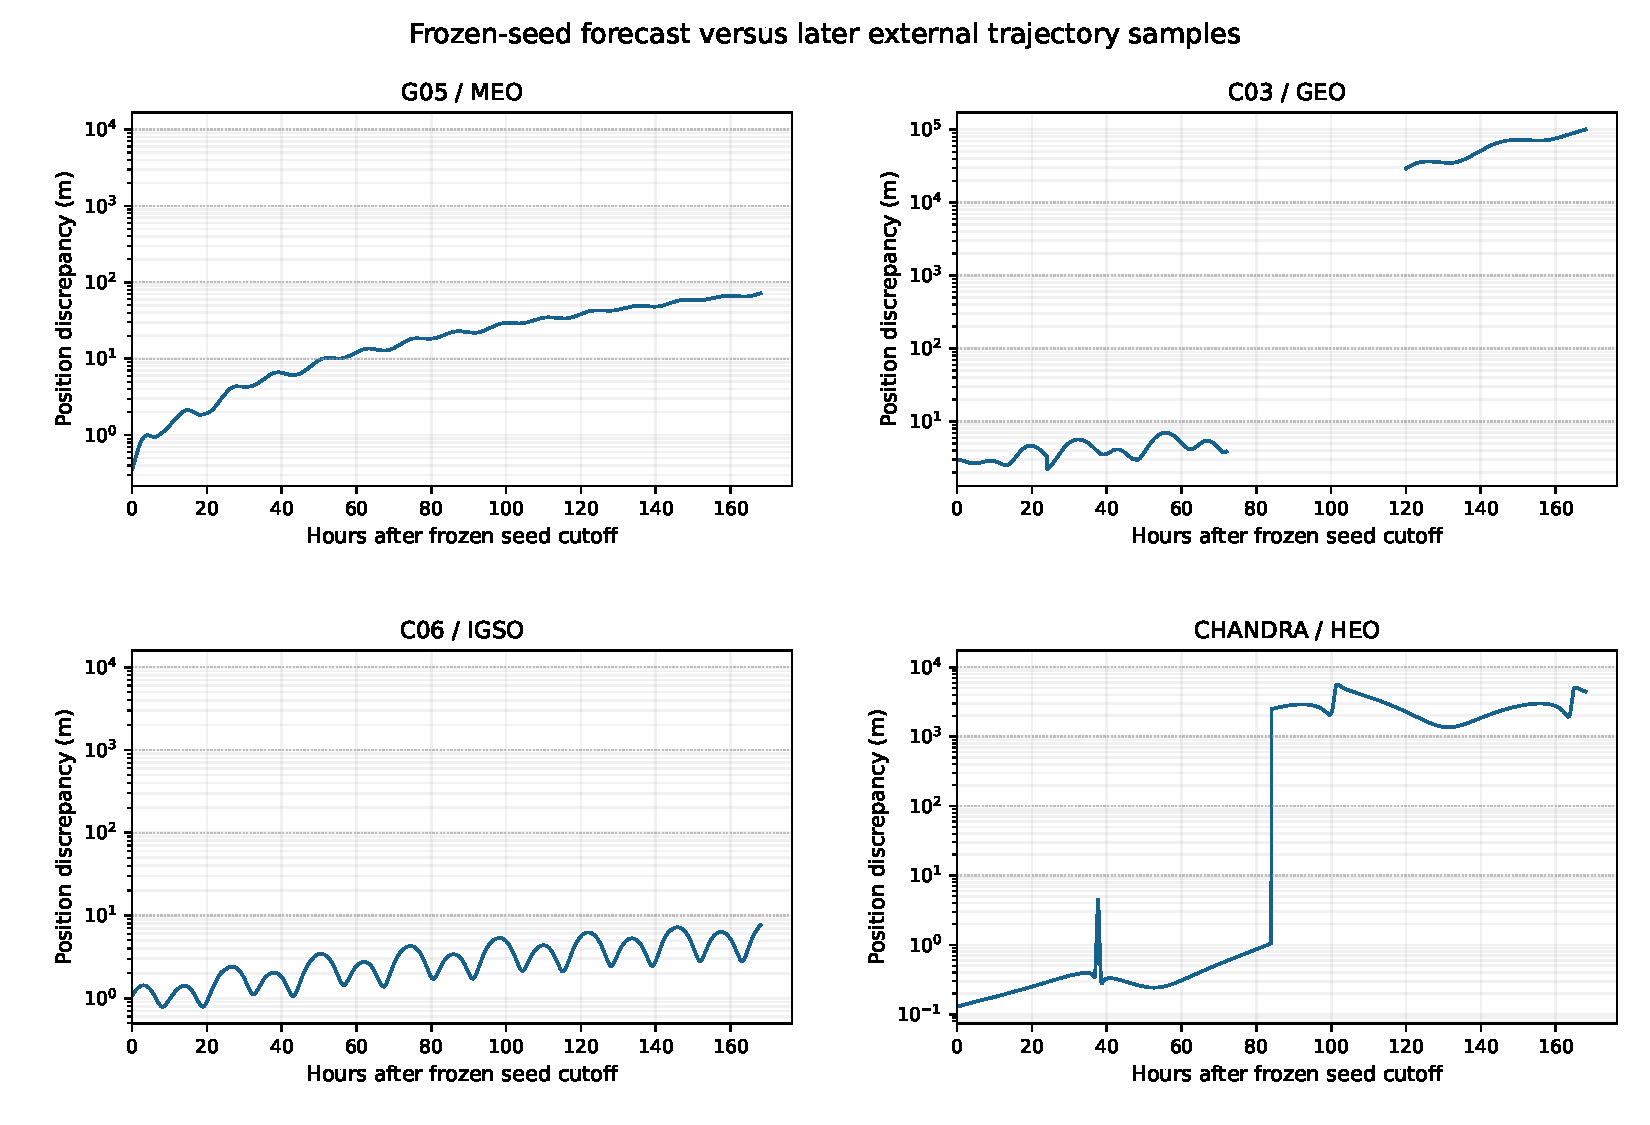
\includegraphics[width=\linewidth]{../results/orbit_accuracy_confirmation_cpu_verified/forecast_error_curves.pdf}
\end{center}
The selection rule was frozen before this date's errors were evaluated. The
C03 reference gap is blank; connecting its endpoints would imply unavailable
measurements. Chandra's source discontinuity is retained. Lines join only
available adjacent samples and do not certify error between samples or beyond
the declared window.
